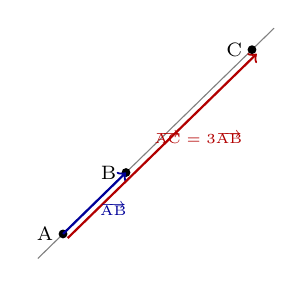
\begin{tikzpicture}[x=4mm,y=2.6mm]
\ax{-0.5}{8}{-0.5}{12}
\draw[gray,domain=0.2:7.7,samples=80] plot (\x,{1.5*\x+0.5});
\fill (1,2) circle (1.6pt);
\node[left] at (1,2){\scriptsize A};
\fill (3,5) circle (1.6pt);
\node[left] at (3,5){\scriptsize B};
\fill (7,11) circle (1.6pt);
\node[left] at (7,11){\scriptsize C};
\draw[->,thick,blue!60!black] (1,2)--(3,5); \draw[->,thick,red!70!black] (1.15,1.8)--(7.15,10.8); \node[blue!60!black] at (2.6,3.2){\tiny $\overrightarrow{\mathrm{AB}}$}; \node[red!70!black] at (5.3,6.7){\tiny $\overrightarrow{\mathrm{AC}}=3\overrightarrow{\mathrm{AB}}$};
\end{tikzpicture}